\chapter{Screenshots}
\label{appendix:screenshots}

\begin{figure}[H]
	\centering
	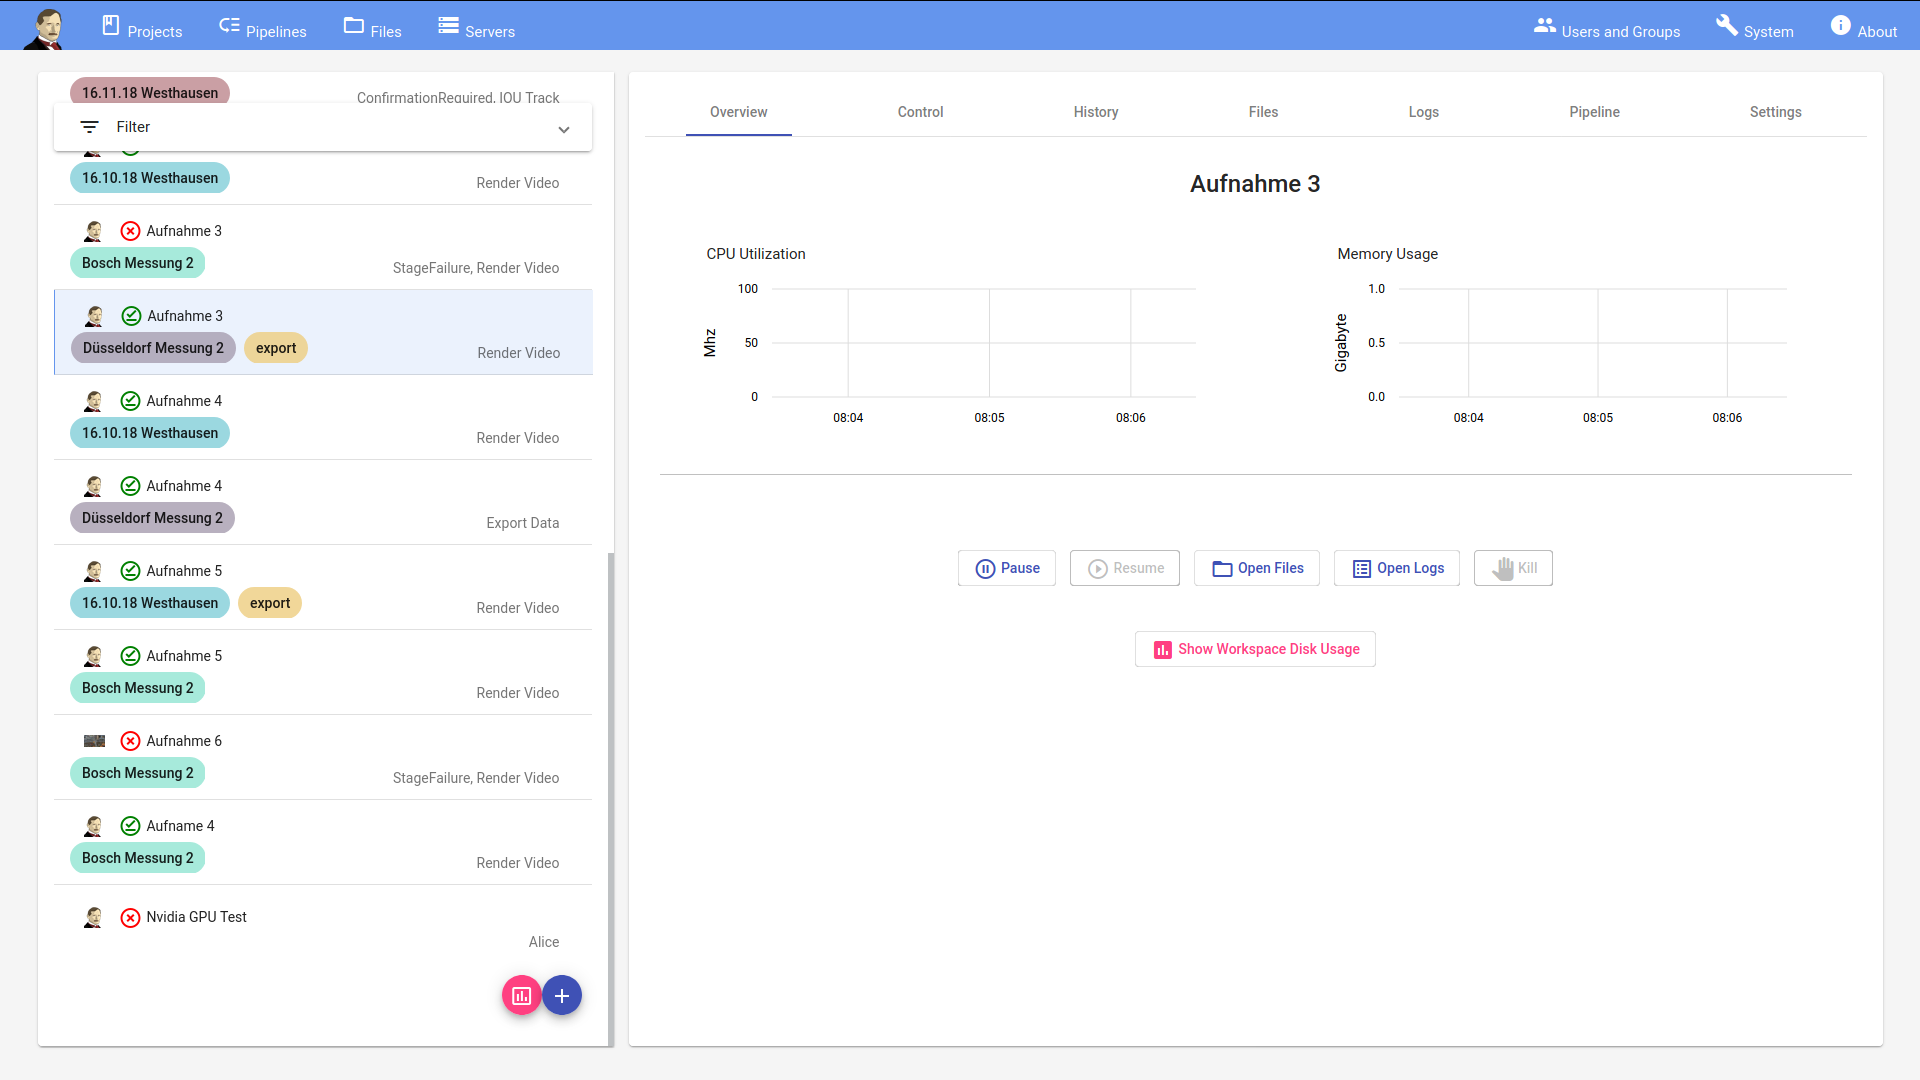
\includegraphics[width=1.0\textwidth]{screenshots/01_project_overview.png}
	\caption{Left: Known projects, Right: Overview for the selected project}
\end{figure}

\begin{figure}[H]
	\centering
	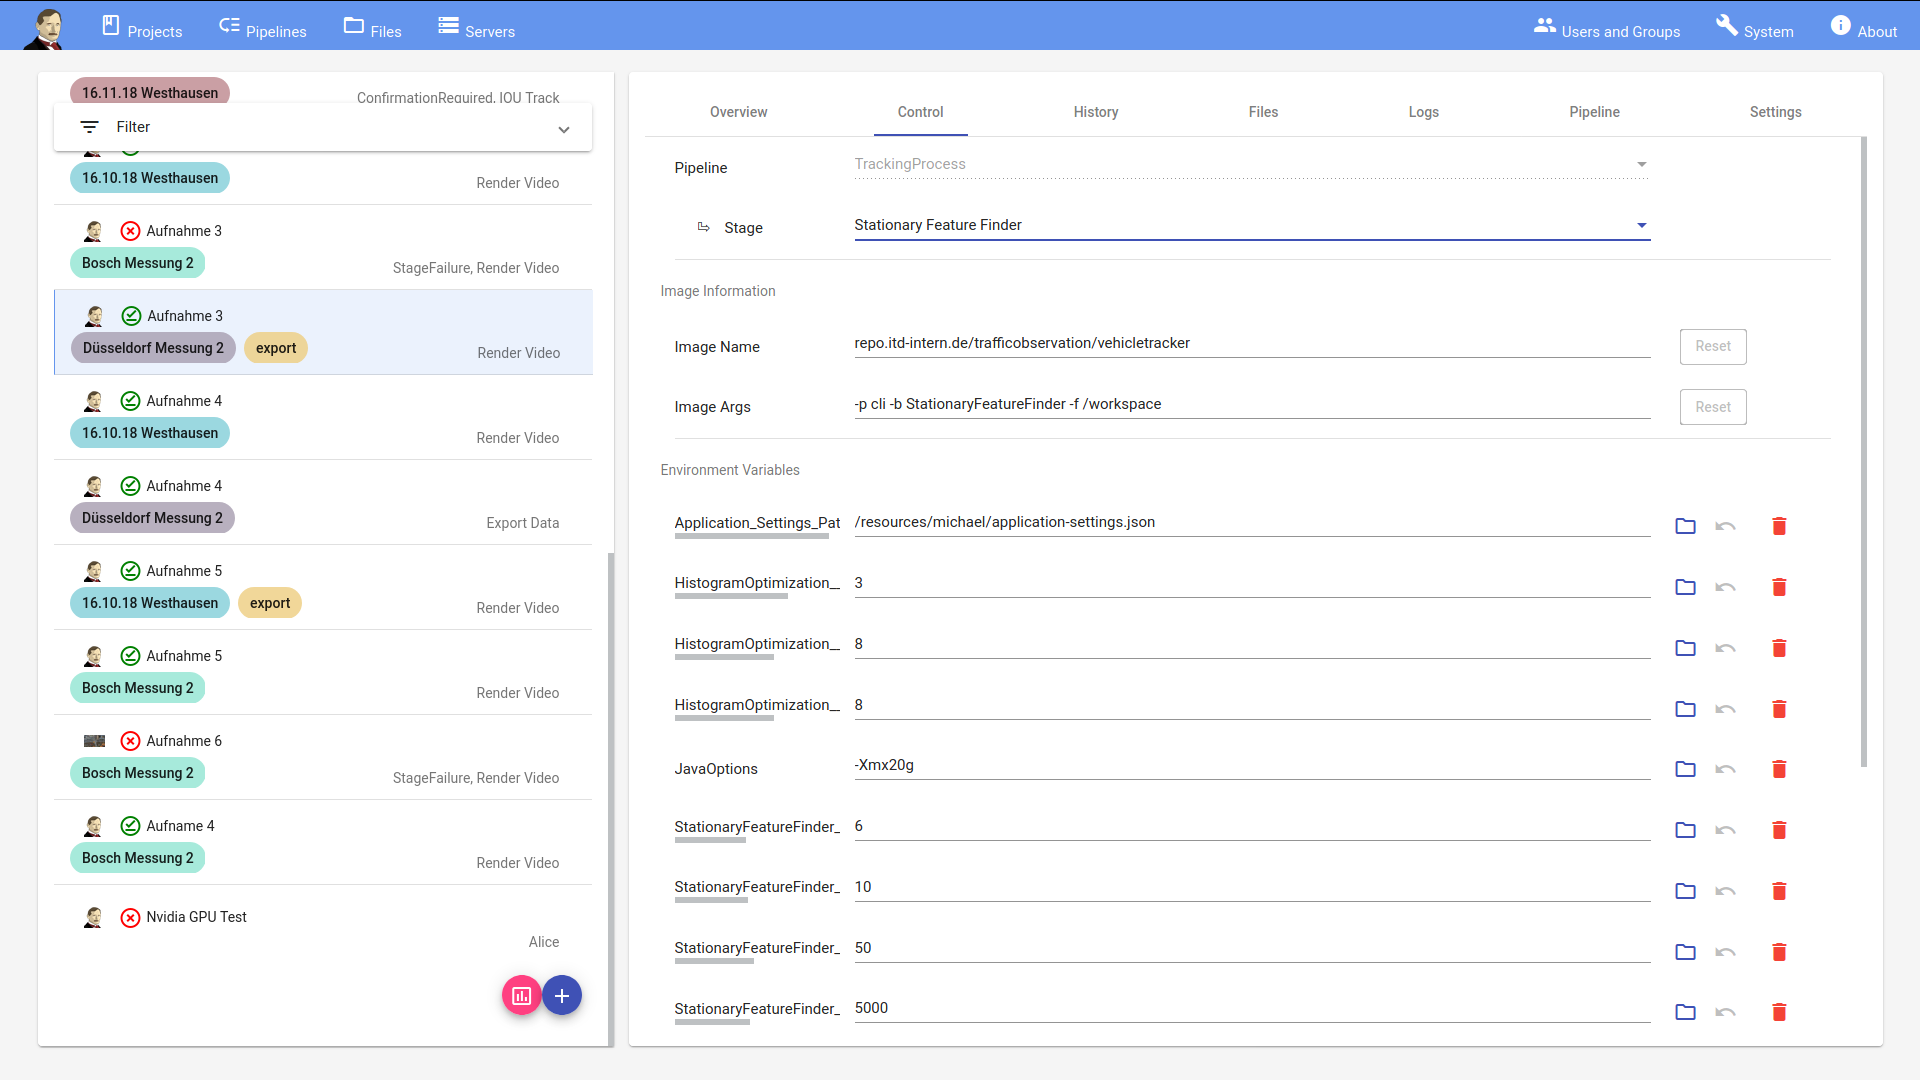
\includegraphics[width=1.0\textwidth]{screenshots/02_project_control.png}
	\caption{Left: Known projects, Right: Control for the selected project}
\end{figure}

\begin{figure}[H]
	\centering
	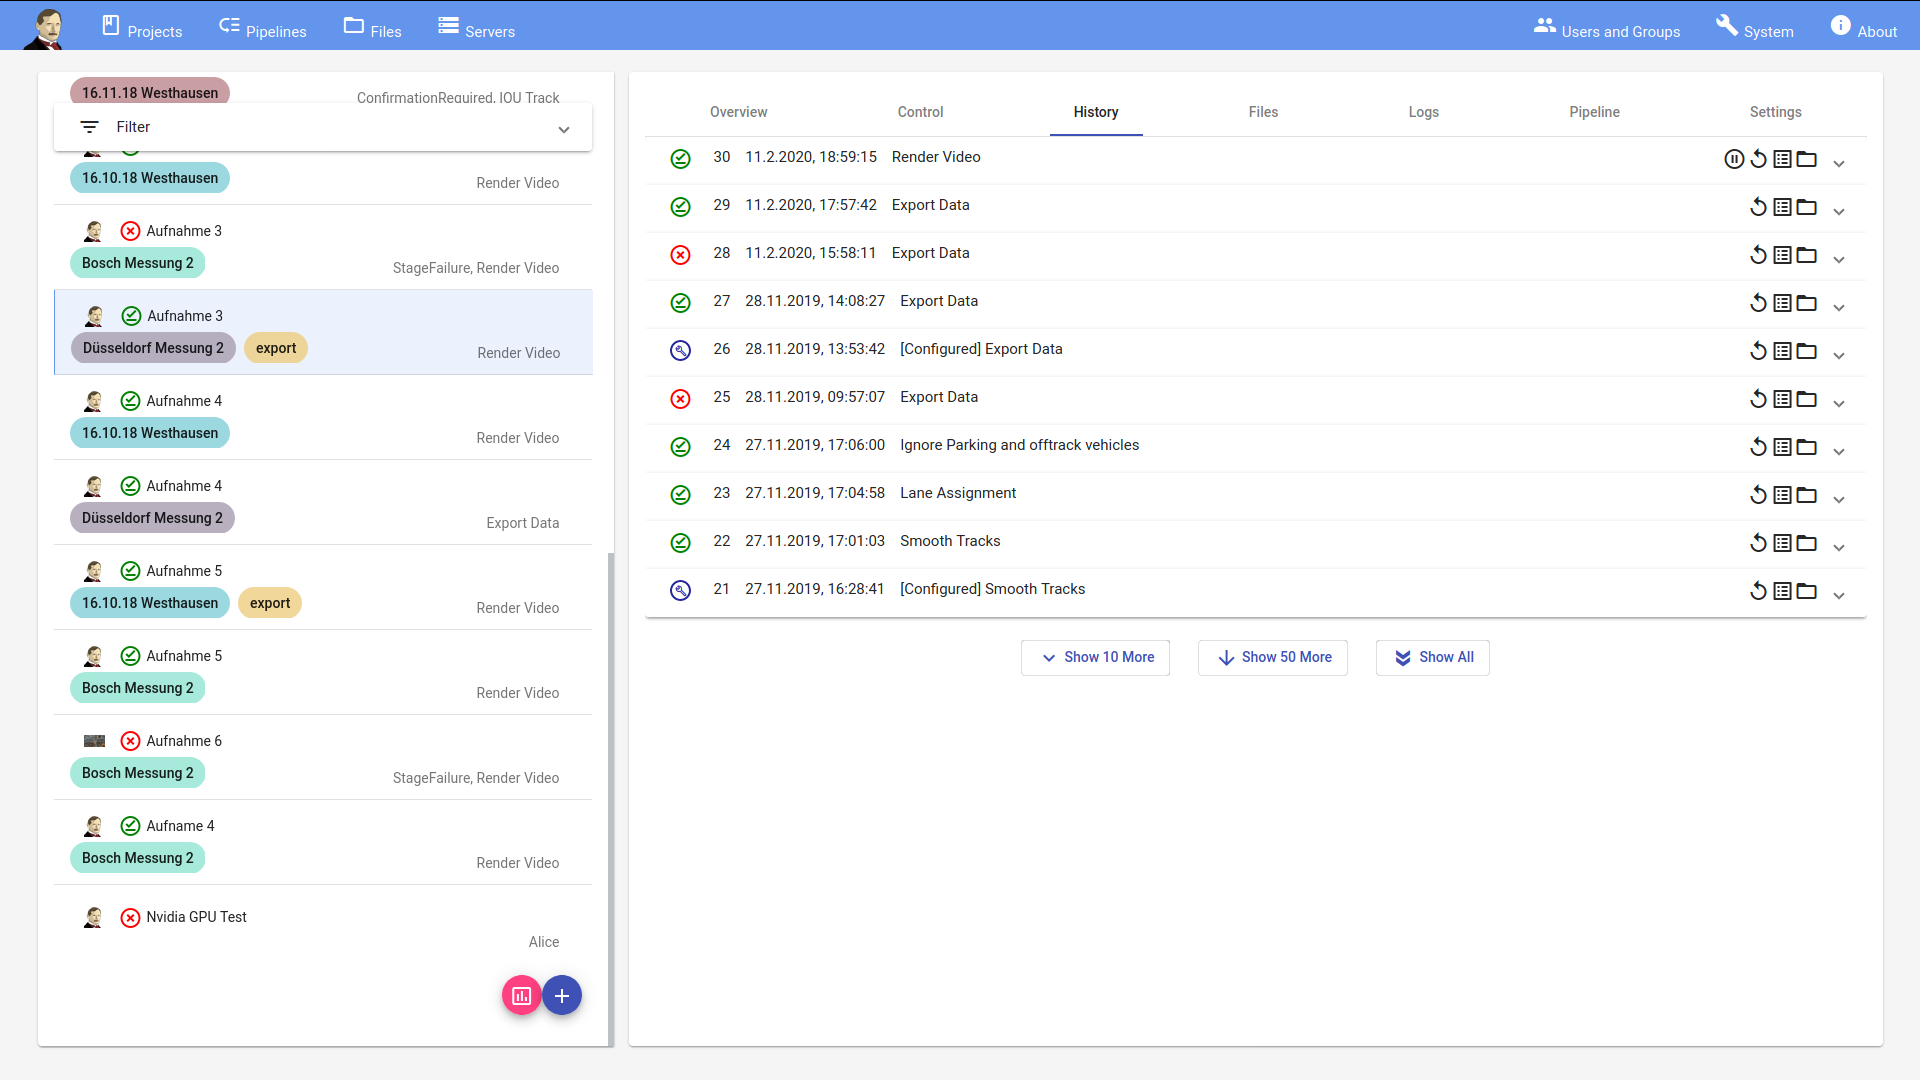
\includegraphics[width=1.0\textwidth]{screenshots/03_project_history.png}
	\caption{Left: Known projects, Right: History of the selected project}
\end{figure}

\begin{figure}[H]
	\centering
	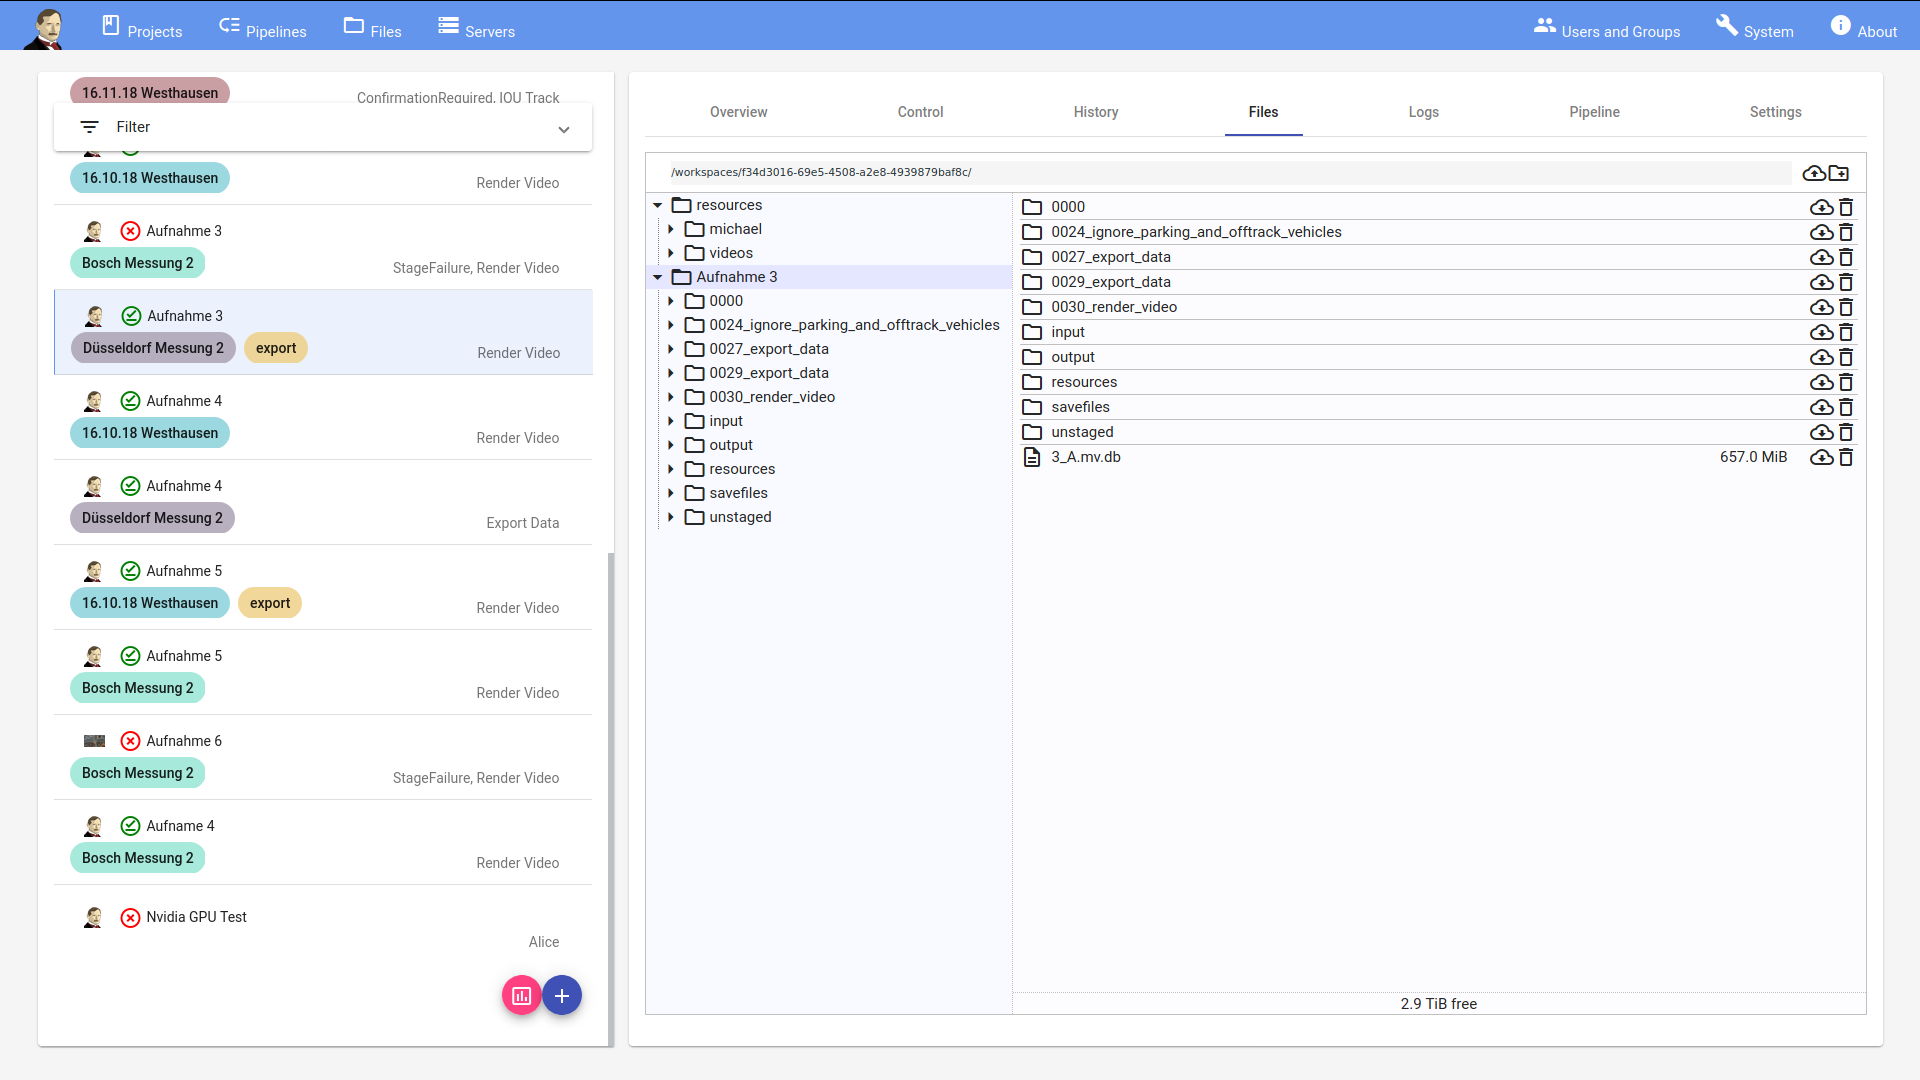
\includegraphics[width=1.0\textwidth]{screenshots/04_project_files.png}
	\caption{Left: Known projects, Right: Files associated with the selected project}
\end{figure}

\begin{figure}[H]
	\centering
	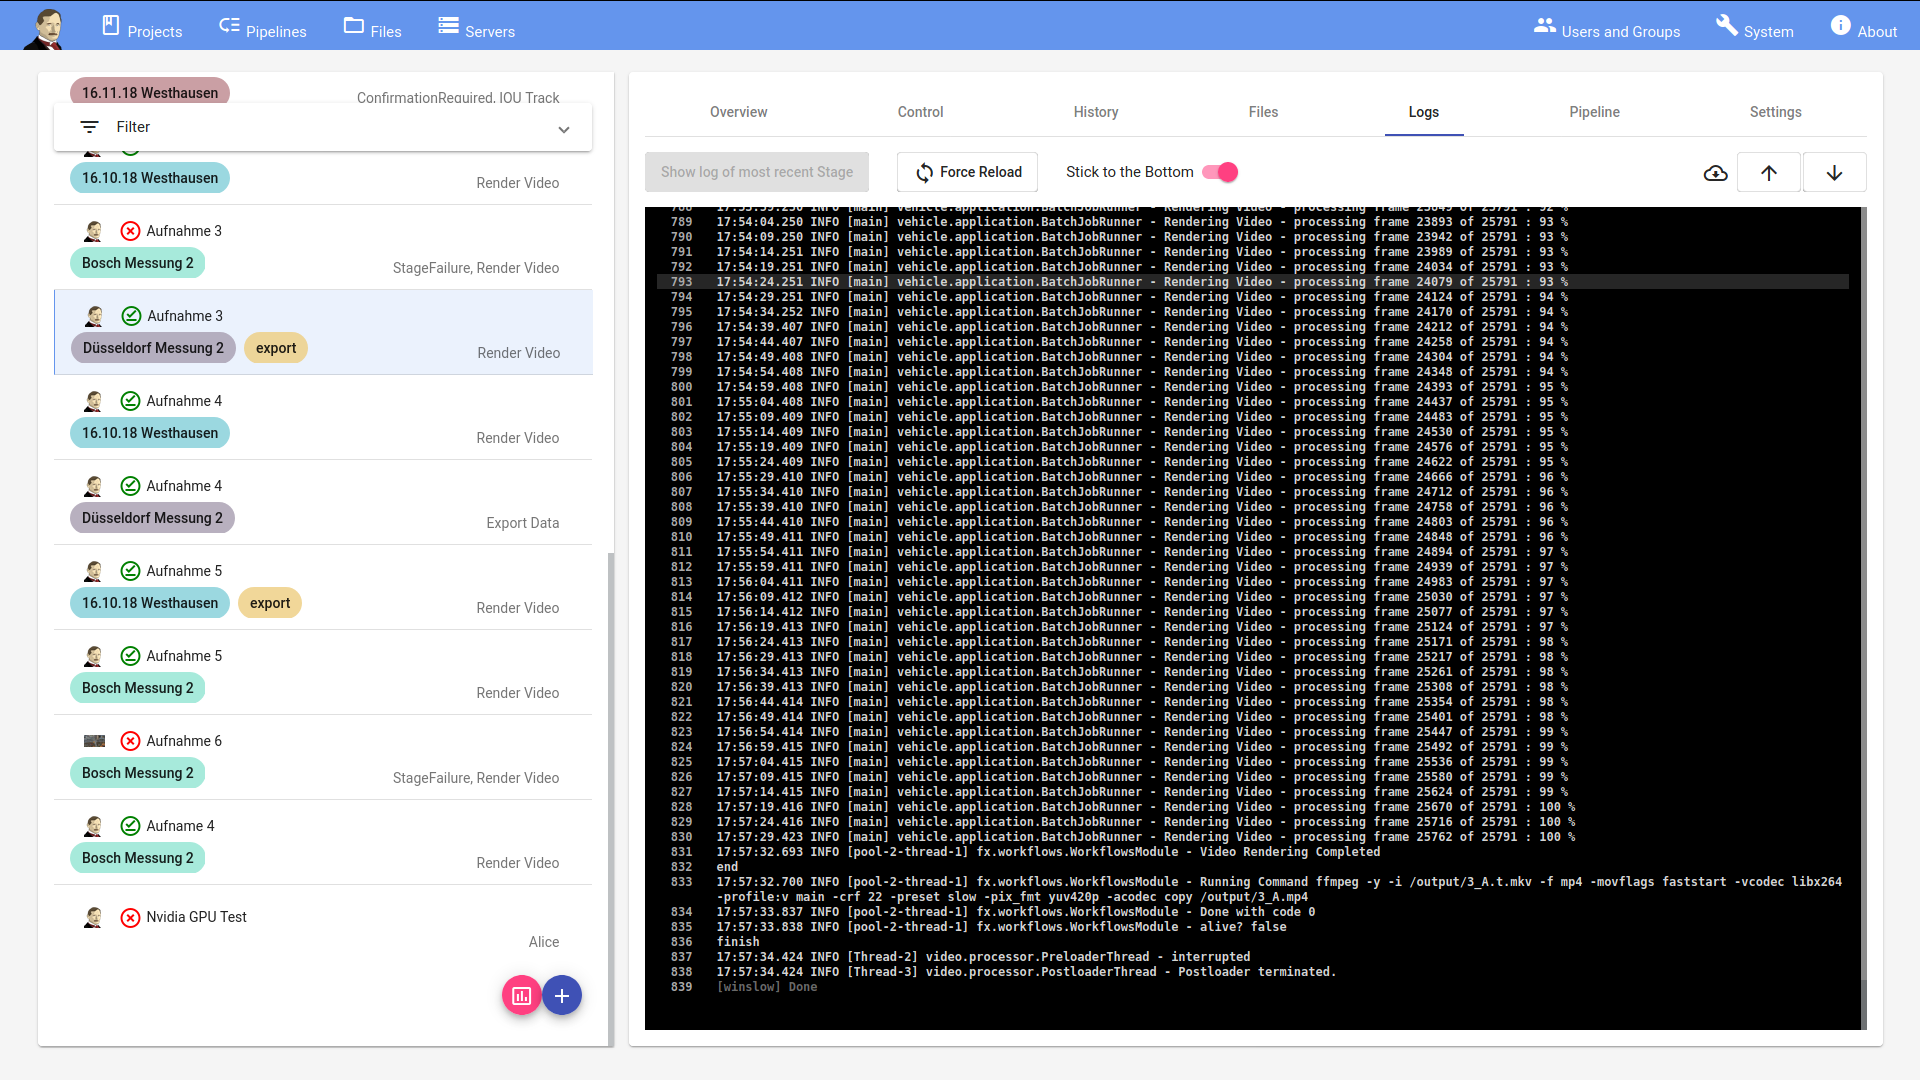
\includegraphics[width=1.0\textwidth]{screenshots/05_project_logs.png}
	\caption{Left: Known projects, Right: Most recent logs for the selected project}
\end{figure}

\begin{figure}[H]
	\centering
	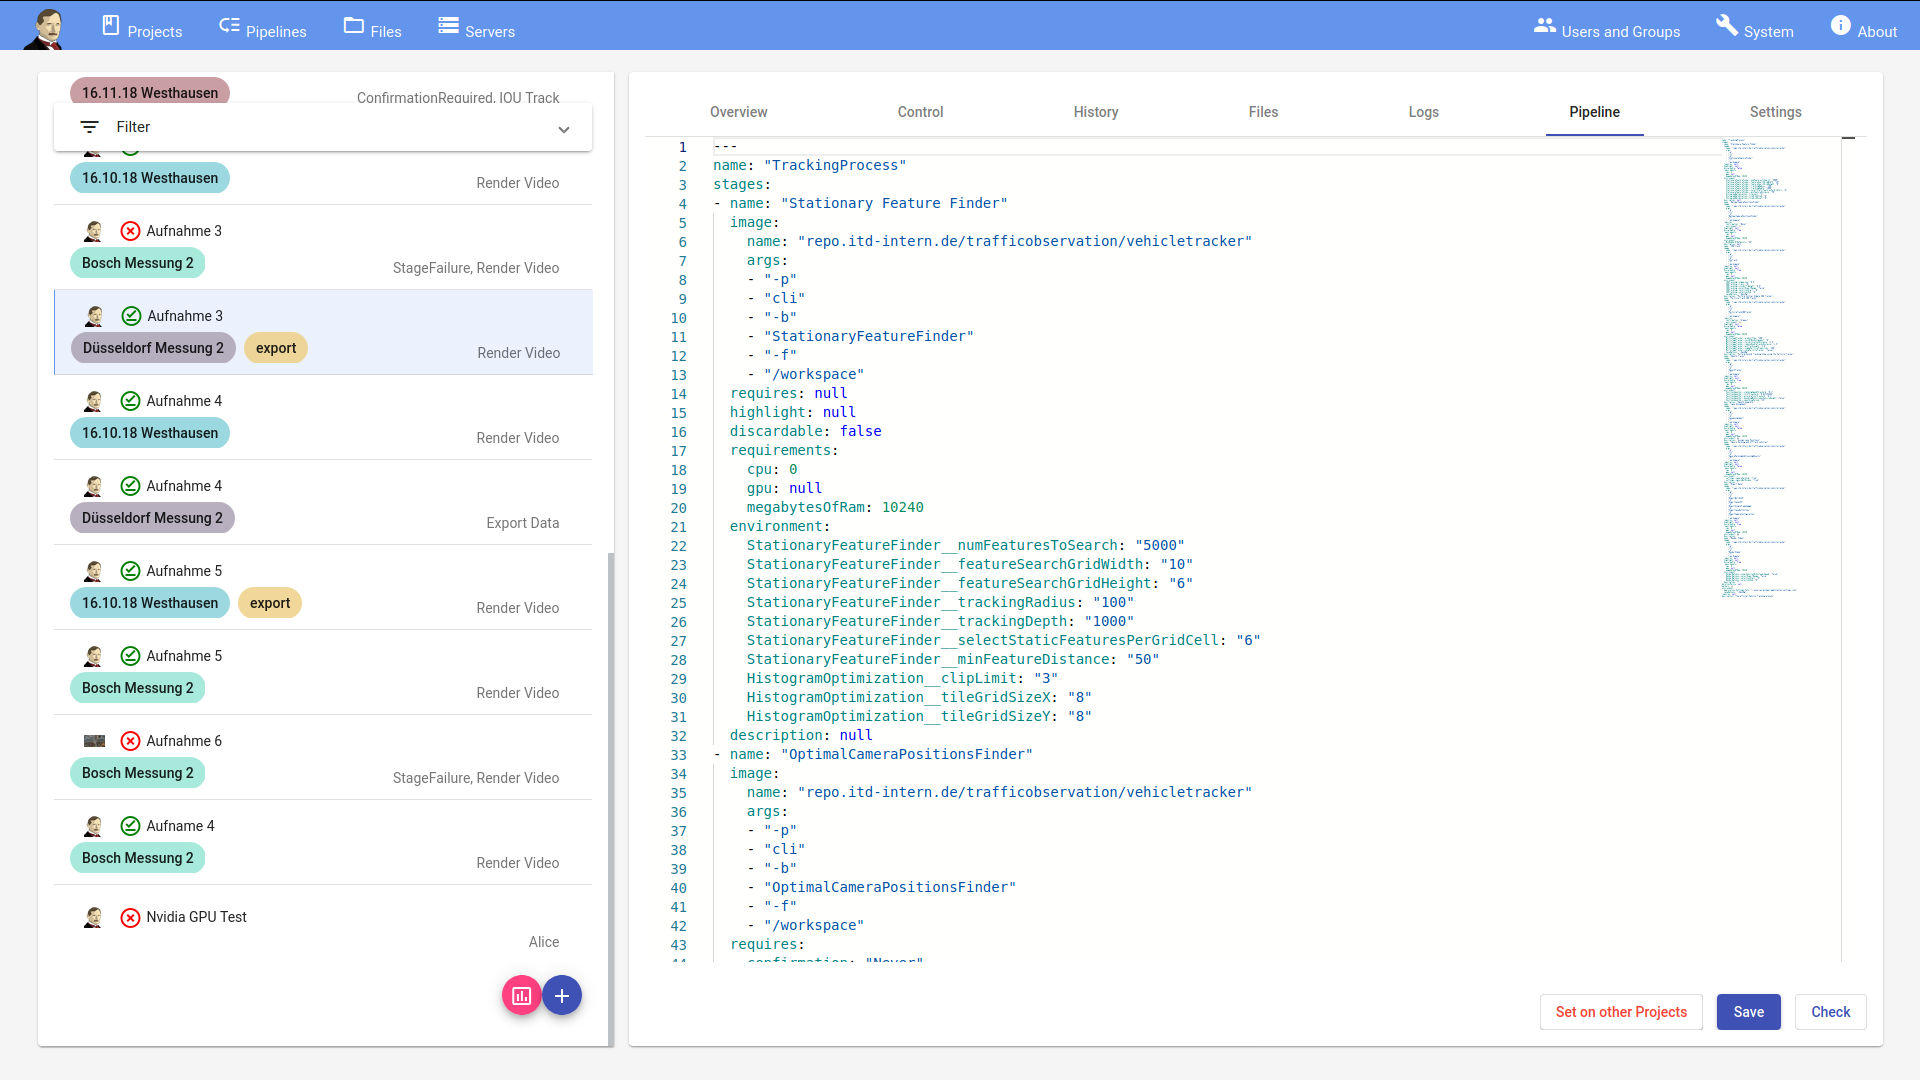
\includegraphics[width=1.0\textwidth]{screenshots/06_project_pipeline.png}
	\caption{Left: Known projects, Right: Pipeline of the selected project}
\end{figure}

\begin{figure}[H]
	\centering
	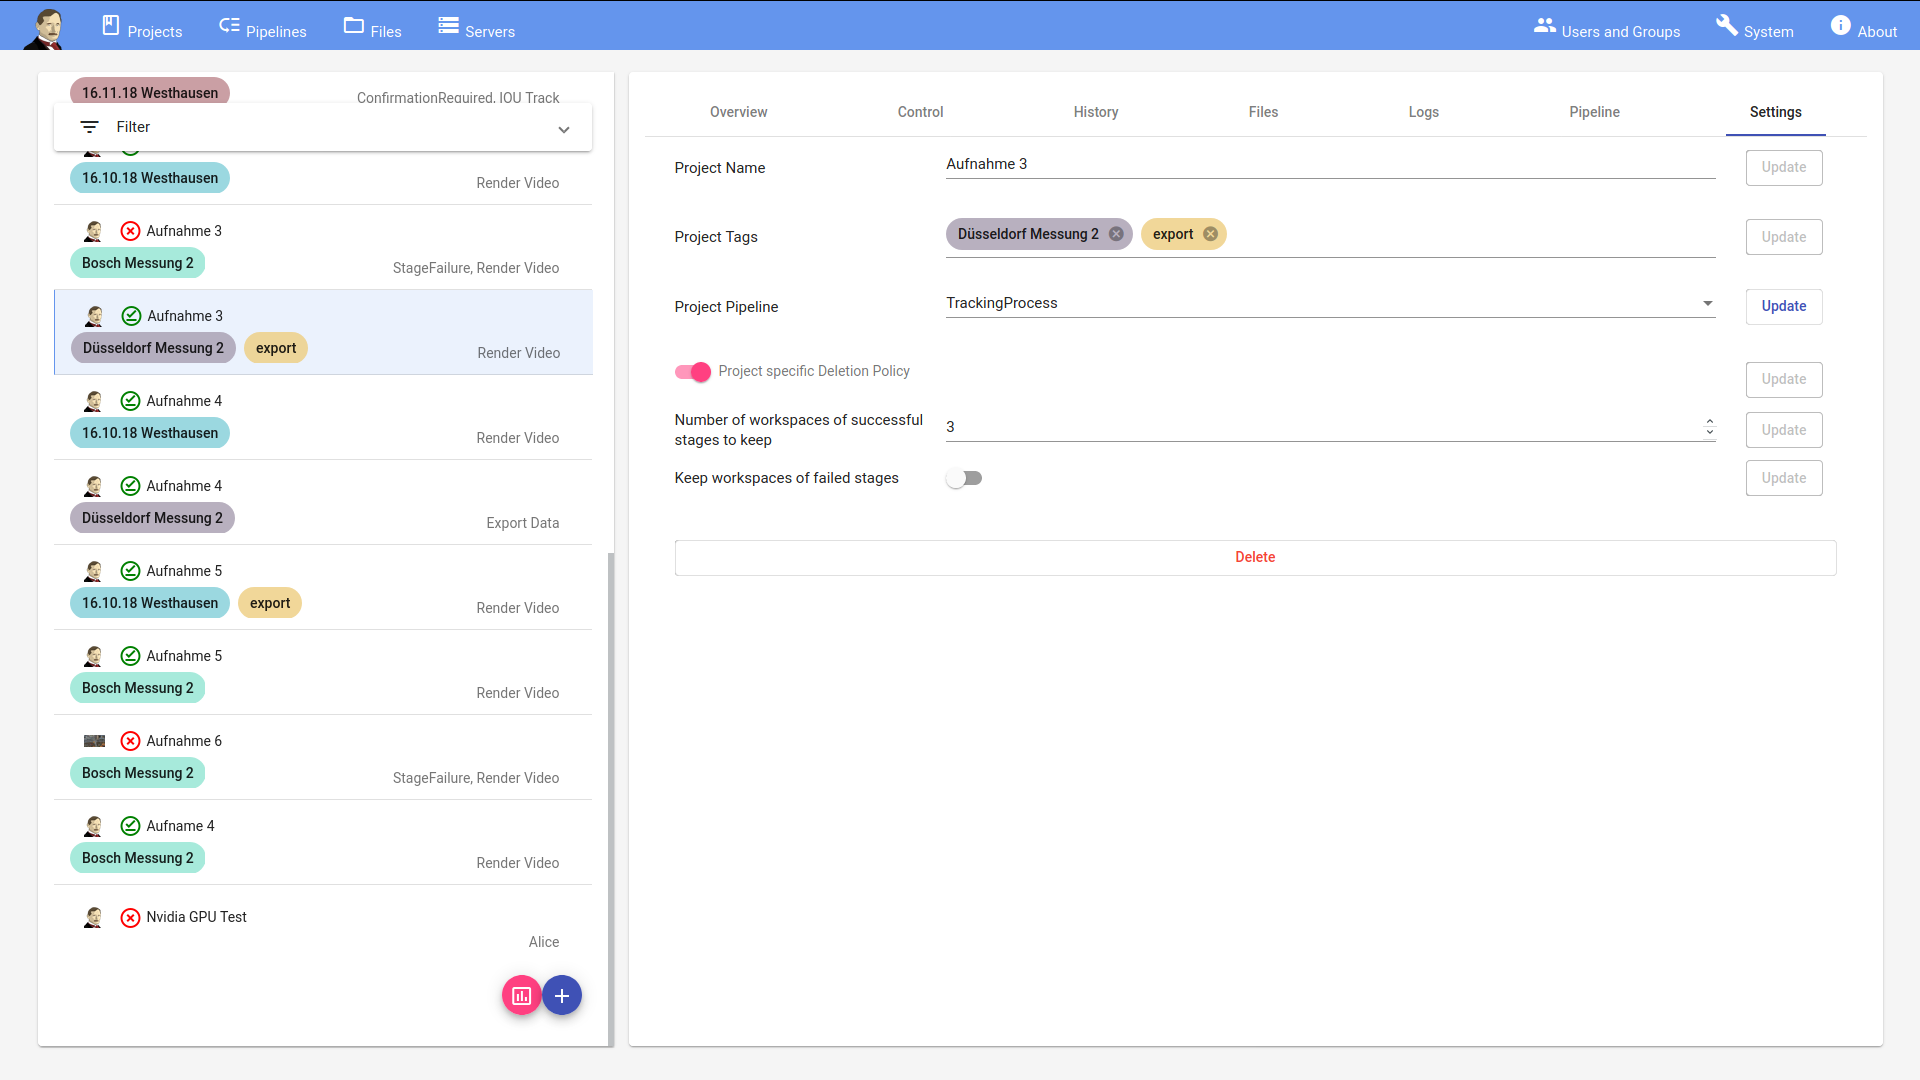
\includegraphics[width=1.0\textwidth]{screenshots/07_project_settings.png}
	\caption{Left: Known projects, Right: Settings of the selected project}
\end{figure}

\begin{figure}[H]
	\centering
	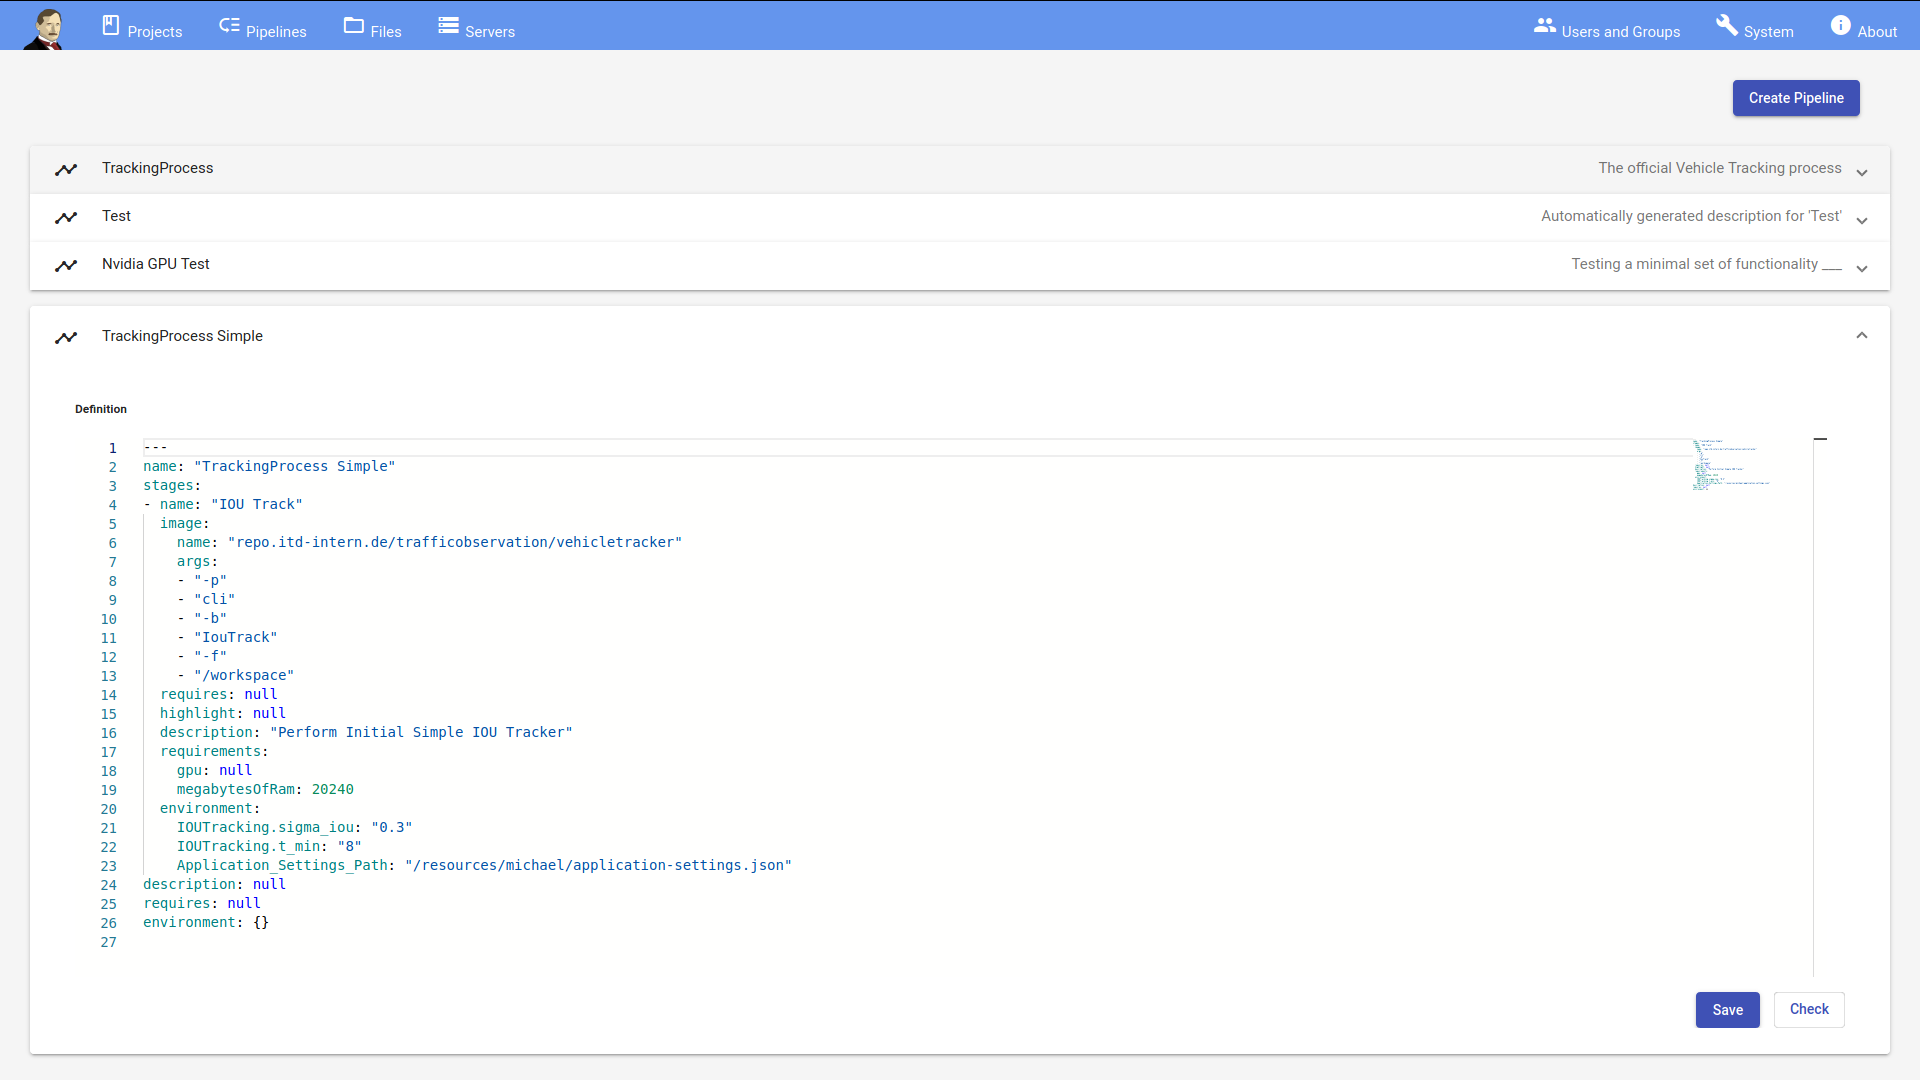
\includegraphics[width=1.0\textwidth]{screenshots/08_pipelines.png}
	\caption{Edit view for pipeline definitions}
\end{figure}

\begin{figure}[H]
	\centering
	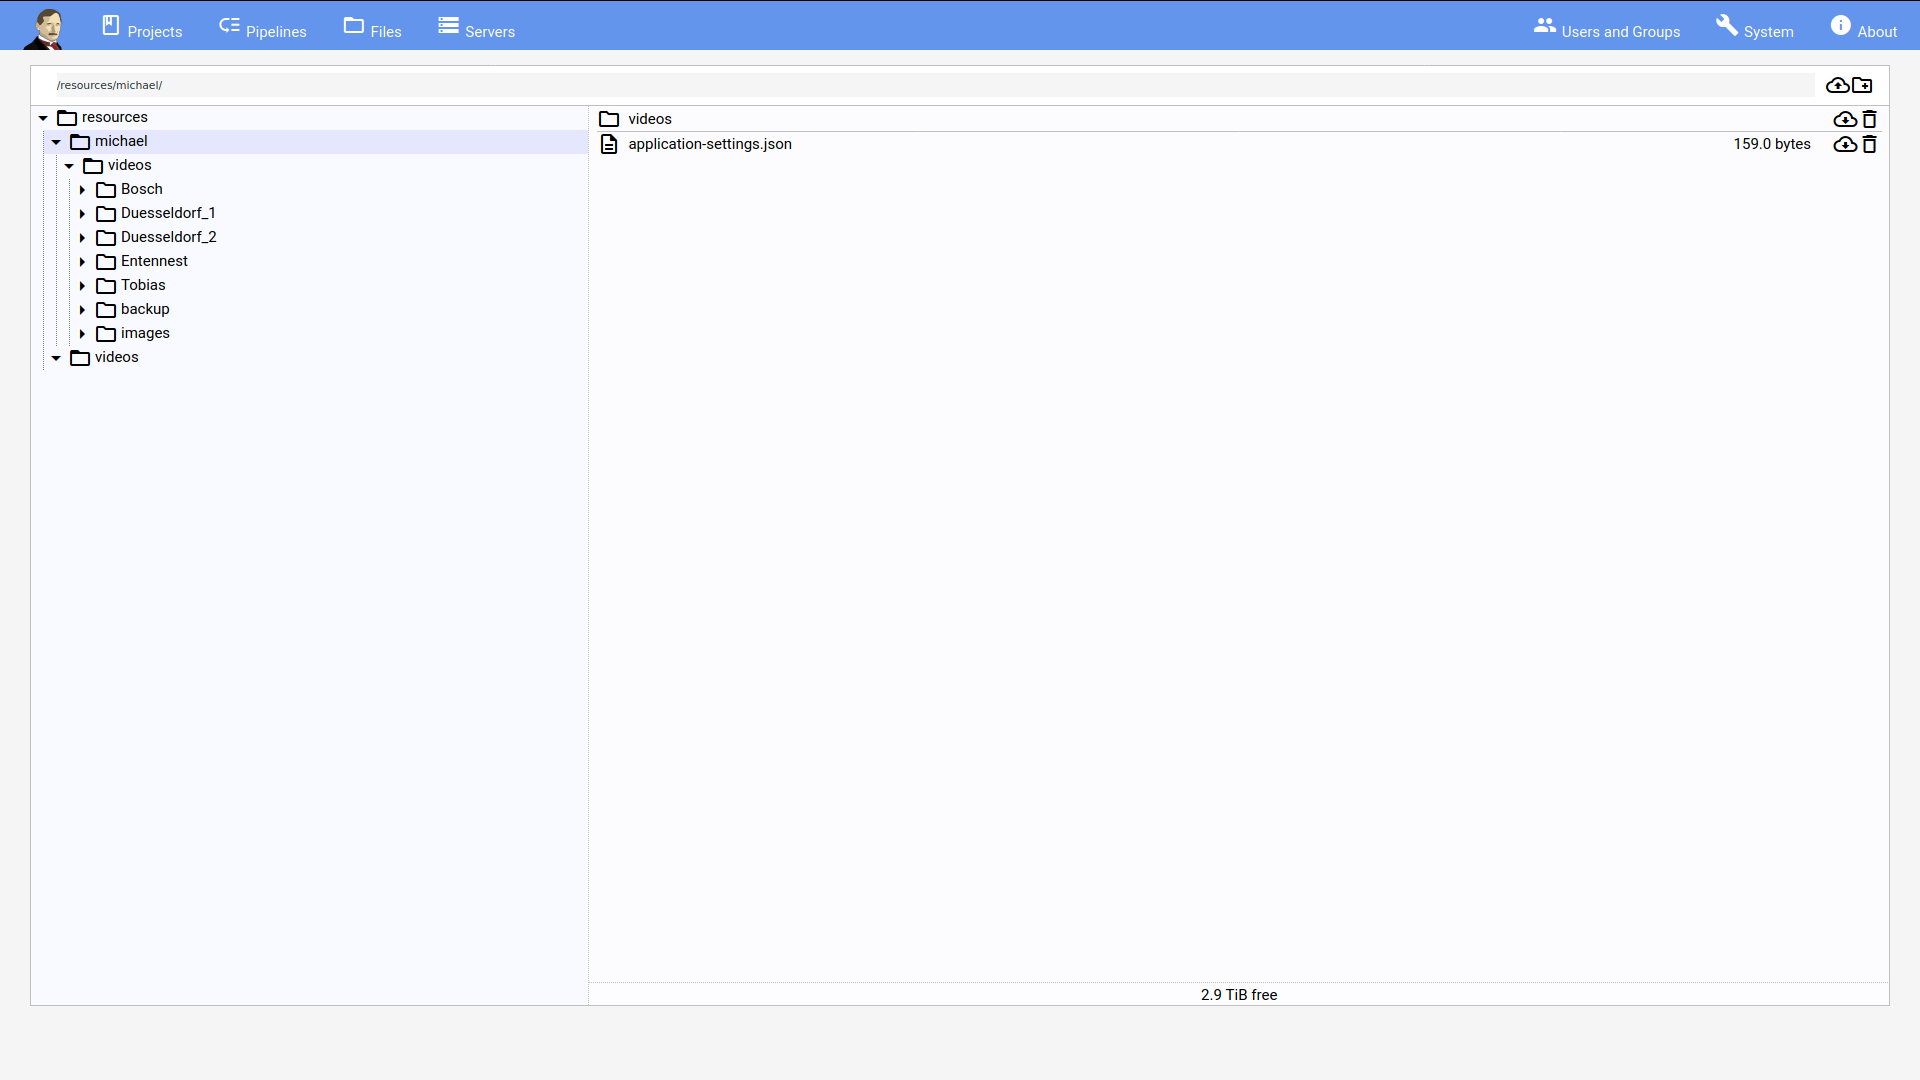
\includegraphics[width=1.0\textwidth]{screenshots/09_files.png}
	\caption{File explorer which is not restricted to a project}
\end{figure}

\begin{figure}[H]
	\centering
	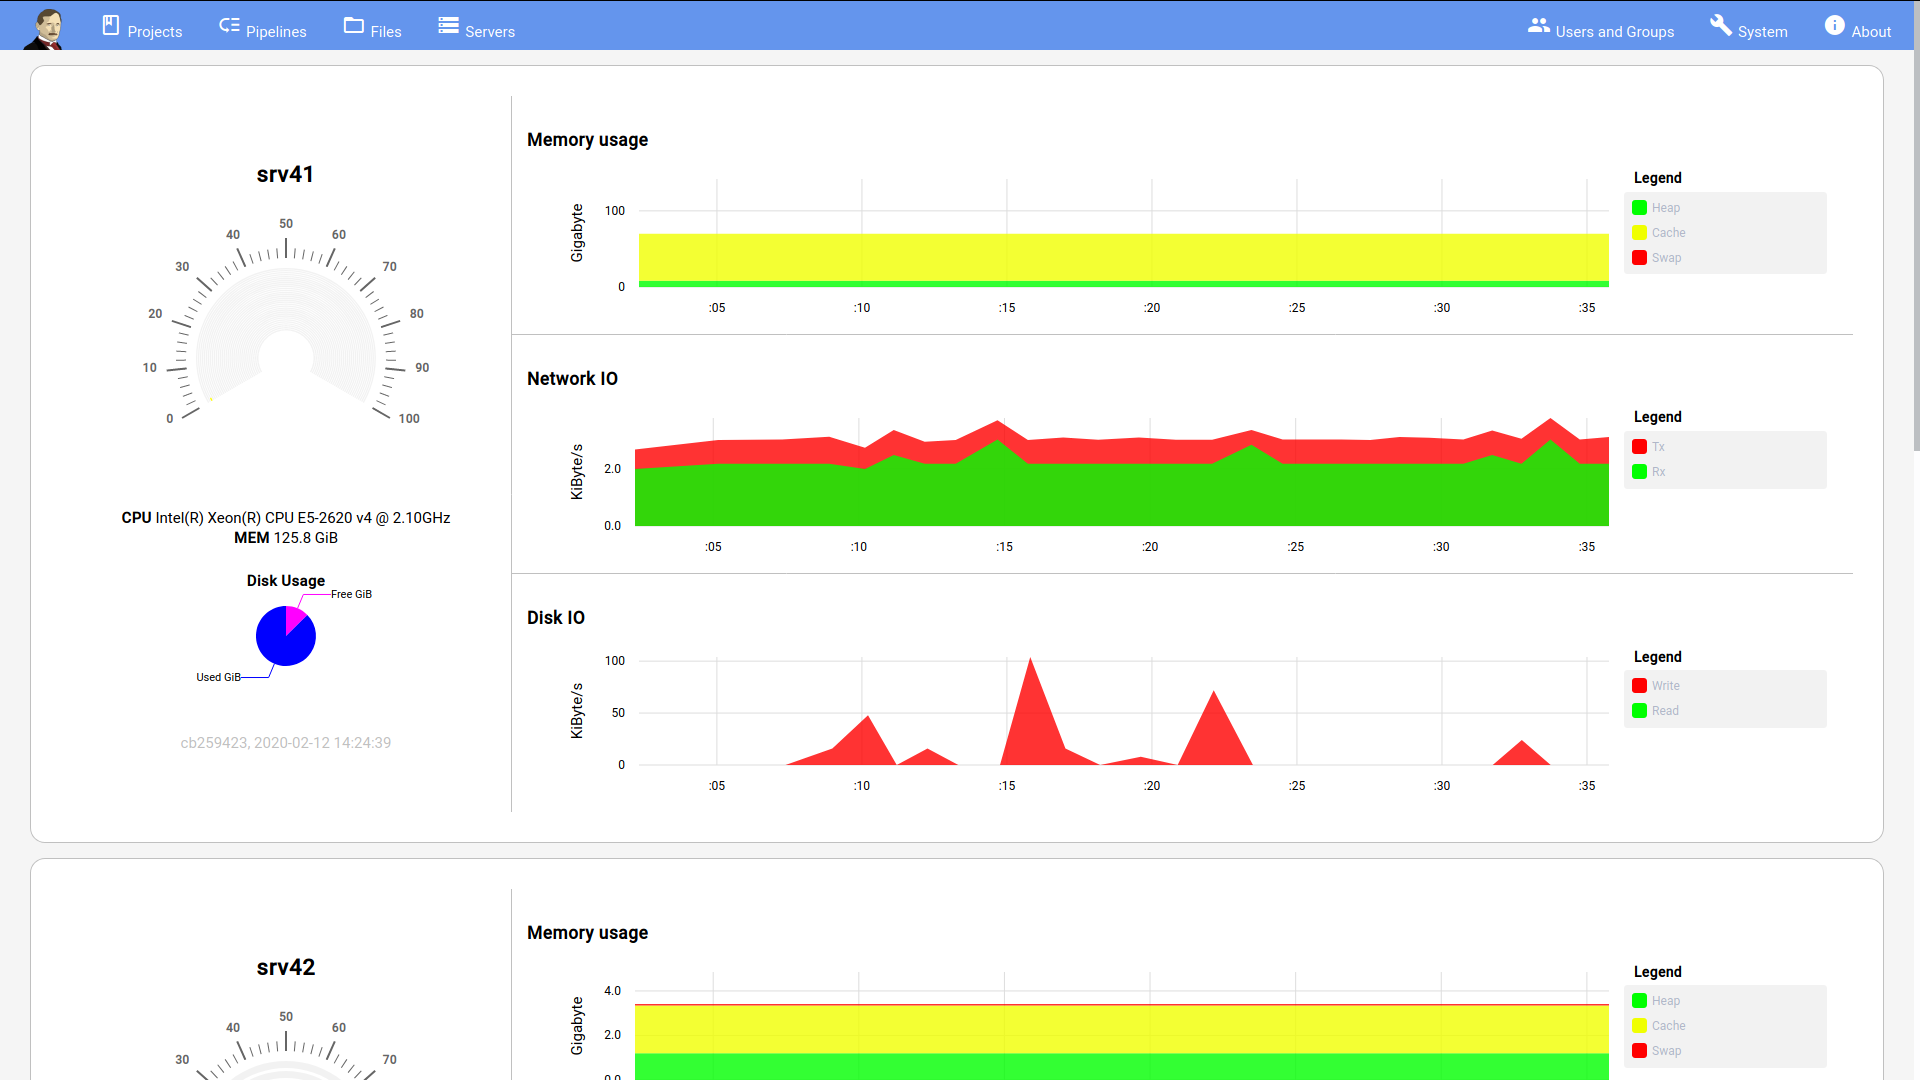
\includegraphics[width=1.0\textwidth]{screenshots/10_servers_1.png}
	\caption{Utilization overview for every attached Winslow instance}
\end{figure}

\begin{figure}[H]
	\centering
	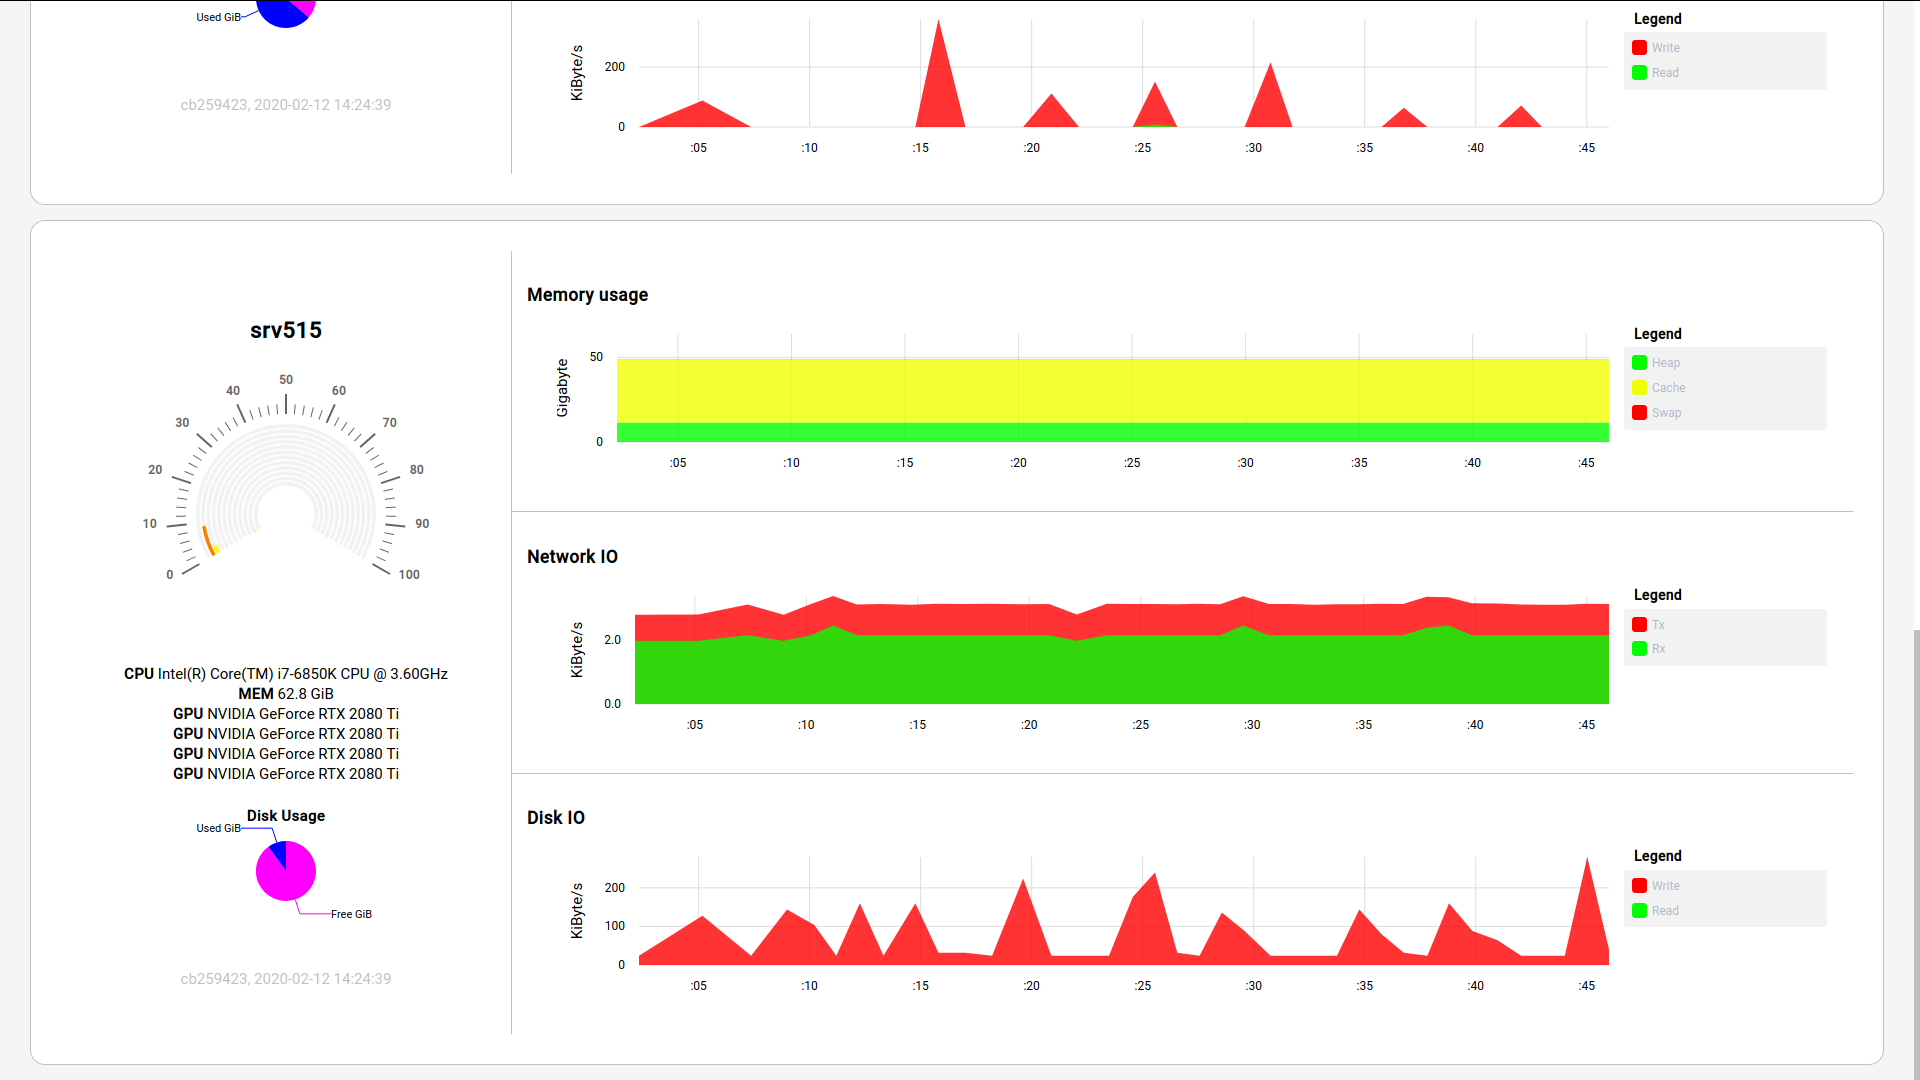
\includegraphics[width=1.0\textwidth]{screenshots/11_servers_2.png}
	\caption{Utilization overview for every attached Winslow instance}
\end{figure}
